\section{Muon ID}

To increase sensitivity to a lower mass Higgs boson, the lepton $p_T$ threshold needs to be lowered. However, background contributions from muon fakes occur more often at lower momenta. The selection requirements from AN-10-344 were optimized for leptons above $20\:\GeVoverc$. This section presents studies on isolation and impact parameter requirements to improve the muon identification performance in the range, $10\:\GeVoverc < p_T < 20\:\GeVoverc$.

The nominal selection is extended to allow for one lepton with $p_T$ down to $10\:\GeVoverc$. The expected yield in $1\:\invfb$ is computed by applying the selection to the Higgs signal sample for mass $130\:\GeVovercsq$ and to all Monte Carlo background samples except $W+$jets. The $W+$jets expectation is derived by applying the fake rate method on the $W+$jets Monte Carlo sample and the details are explained in a later sub-section. The reason for the unique treatment of $W+$jets is because too few events remain after applying selection on the $W+$jets Monte Carlo, and too few tight-loose candidates are found in data to make a useful extrapolation. The nominal yield expectations for the $e\mu$ and $\mu\mu$ final states are listed in Table~\ref{tab:muidyield0}, where the trailing lepton is a muon.

\begin{table}[!htbp]
\begin{center}
\begin{tabular}{|l|c|c|c|}
\hline
	Source & $p_T > 20$ & $15 < p_T < 20$ & $10 < p_T < 15$ \\
\hline
$H\rightarrow WW$ ($e\mu$) & $2.428$  & $1.587$ & $1.305$ \\
$W+$jets ($e+$fake $\mu$)  & $0$      & $0.77$  & $2.64$ \\
Other backgrounds($e\mu$)  & $12.167$ & $6.325$ & $4.161$ \\
\hline
$H\rightarrow WW$ ($\mu\mu$) & $2.553$  & $1.399$ & $1.047$ \\
$W+$jets ($\mu$+fake $\mu$)  & $0.11$   & $1.94$  & $1.20$ \\
Other backgrounds($\mu\mu$)  & $13.664$ & $7.576$ & $3.647$ \\
\hline
\end{tabular}
\caption{Predicted yields for $1\:\invfb$ in the $e\mu$ and $\mu\mu$ final states with the nominal selection extended to allow a lepton leg down to $10\:\GeVoverc$.}
\label{tab:muidyield0}
\end{center}
\end{table}

\subsection{Fake Rate Method}
The fake rate method is applied for two purposes in this study. As discussed above, the method is applied to the $W+$jets Monte Carlo sample to extract a yield for lepton plus muon fake events. The method is also applied to the data to determine how the fake rate varies with changing the isolation and impact parameter requirements. The relative change of the fake rate in data is then used to re-scale the Monte Carlo prediction.

The fakeable object is defined as a GlobalMuon satisfying,
\begin{itemize}
\item TrackerMuon reconstruction,
\item at least $11$ tracker hits,
\item global fit $\chi^2/$NDF $< 10$,
\item at least $1$ valid muon hit in the global fit,
\item $(I_{trk}+I_{ECAL}+I_{HCAL})/p_T < 1$,
\item $d_0 < 0.2\:$cm with respect to the primary vertex.
\end{itemize}
The event primary vertex is the reconstructed vertex with the highest $\sum p_T^2$ using the Deterministc Annealing algorithm and satisfying standard quality cuts.

In the $W+$jets Monte Carlo, the fakeable object is required to not be within $\Delta R<0.5$ of the generator level muon in the cases of a $W\rightarrow\mu\nu$ event or a $W\rightarrow\tau\nu$ event where the tau decays to a muon, nor be within $\Delta R<0.5$ of the generator level tau in the case of a $W\rightarrow\tau\nu$ event where the tau decays hadronically.

In data, the fakeable object selection must ensure minimal contamination by prompt muons from $W$ and $Z$ decays. The following cuts are applied,
\begin{itemize}
\item $Z$ veto: event is rejected if there are two oppositely charged muons with $p_T>20\:\GeVoverc$ satisfying the fakeable object definition, 
\item $W$ veto: event is rejected if PF-MET $> 20\:\GeV$ or the muon has transverse mass larger than $20\:\GeVovercsq$,
\item there is a PF-jet away from the fakeable object ($\Delta R > 1$) with $p_T>15\:\GeVoverc$ after L2-Relative, L3-Absolute, L2L3-Residual jet corrections and energy density subtraction from the FastJet technique.
\end{itemize}
The motivation for the final criteria listed above is to select events that emulate $W+$jets conditions. The fake rate calibration in data was performed on $5\invpb$ of 2011 data.

\subsection{Figures Of Merit}
As Table~\ref{tab:muidyield0} shows, the background contribution from fakes is not dominant even with the lowered muon $p_T$ requirement. Hence, when tuning the selection cuts on isolation and impact parameter, the objective should not be to reject fakes as much as possible. The performance of the selection criteria is quantified by several figures of merit (FOMs), 
\begin{itemize}
\item $S/B$
\item $S/\sqrt{S+B}$
\item $S/\sqrt{S+B+(\sigma B)^2}$, where $\sigma=0.35$ is the background systematic uncertainty.
\end{itemize}
The FOMs for the nominal selection for the ``20-20'' $p_T$ cuts and for the ``20-10'' $p_T$ cuts are listed in Table~\ref{tab:muidfom0}. It can be seen that just by lowering the $p_T$ threshold, we gain more signal events and we get a substantial increase in the FOMs except for $S/B$. We proceed to study isolation and impact parameter to find an improved working point.

\begin{table}[!htbp]
\begin{center}
\begin{tabular}{|l|c|c|c|}
\hline
	``20-20'' cuts & $e\mu$ & $\mu\mu$ & Both \\
\hline
$S/B$                       & $0.20$ & $0.19$ & $0.19$ \\
$S/\sqrt{S+B}$              & $0.64$ & $0.63$ & $0.90$ \\
$S/\sqrt{S+B+(\sigma B)^2}$ & $0.42$ & $0.41$ & $0.47$ \\
\hline\hline
	``20-10'' cuts & $e\mu$ & $\mu\mu$ & Both \\
\hline
$S/B$                       & $0.20$ & $0.18$ & $0.19$ \\
$S/\sqrt{S+B}$              & $0.95$ & $0.87$ & $1.29$ \\
$S/\sqrt{S+B+(\sigma B)^2}$ & $0.50$ & $0.44$ & $0.50$ \\
\hline
\end{tabular}
\caption{FOMs for the ``20-20'' and ``20-10'' selection using muon identification criteria of AN-10-344.}
\label{tab:muidfom0}
\end{center}
\end{table}

\subsection{Isolation}
We consider varying the isolation cut from the nominal value of $0.15$ down to $0.05$. The curves of fake rate versus signal muon efficiency are shown in Figure~\ref{fig:isoscan}. The signal muon efficiency here is defined as the efficiency to pass full selection, with the modified isolation cut, with respect to a reconstructed muon passing the fakeable object requirements and matched to the generator level muon from $H\rightarrow WW$.

\begin{figure}[!htbp]
\begin{center}
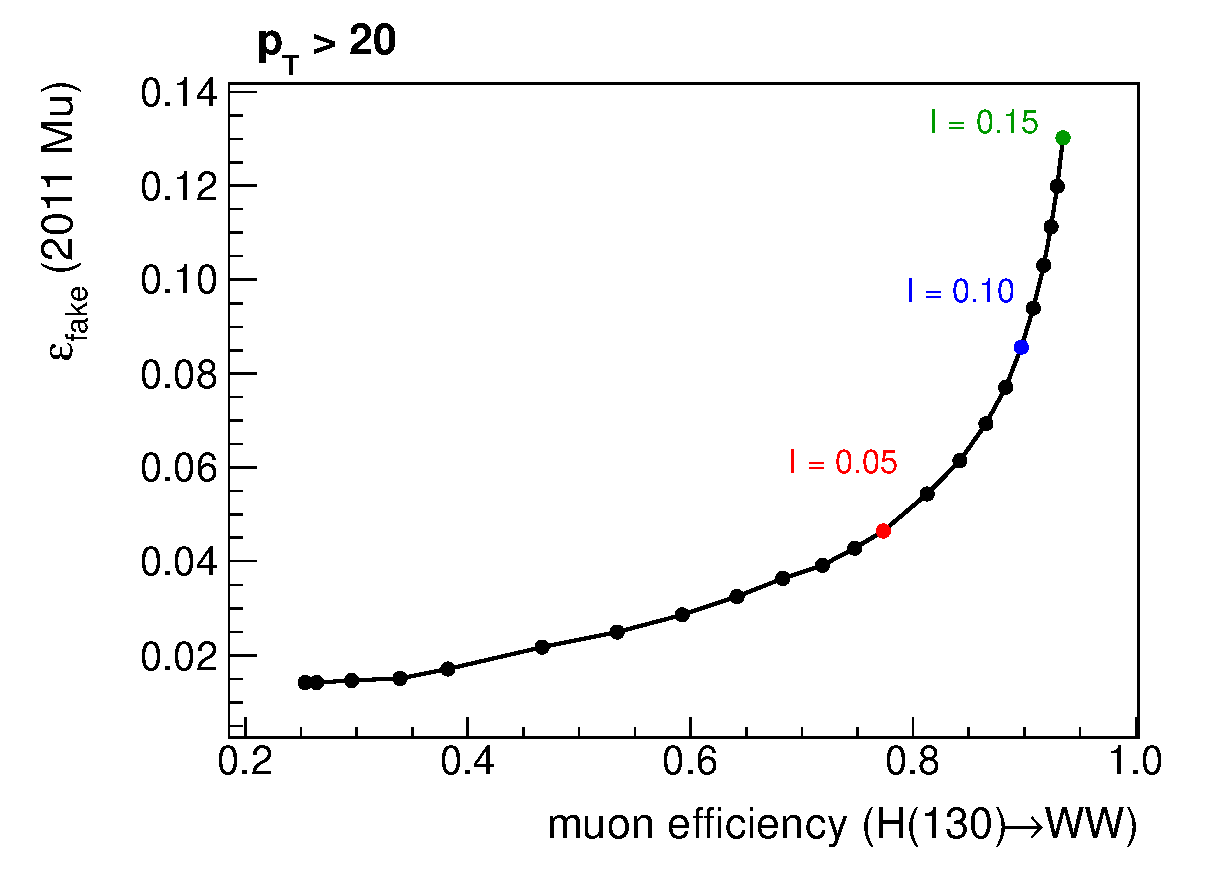
\includegraphics[scale=0.4]{figures/isoscan0.eps}
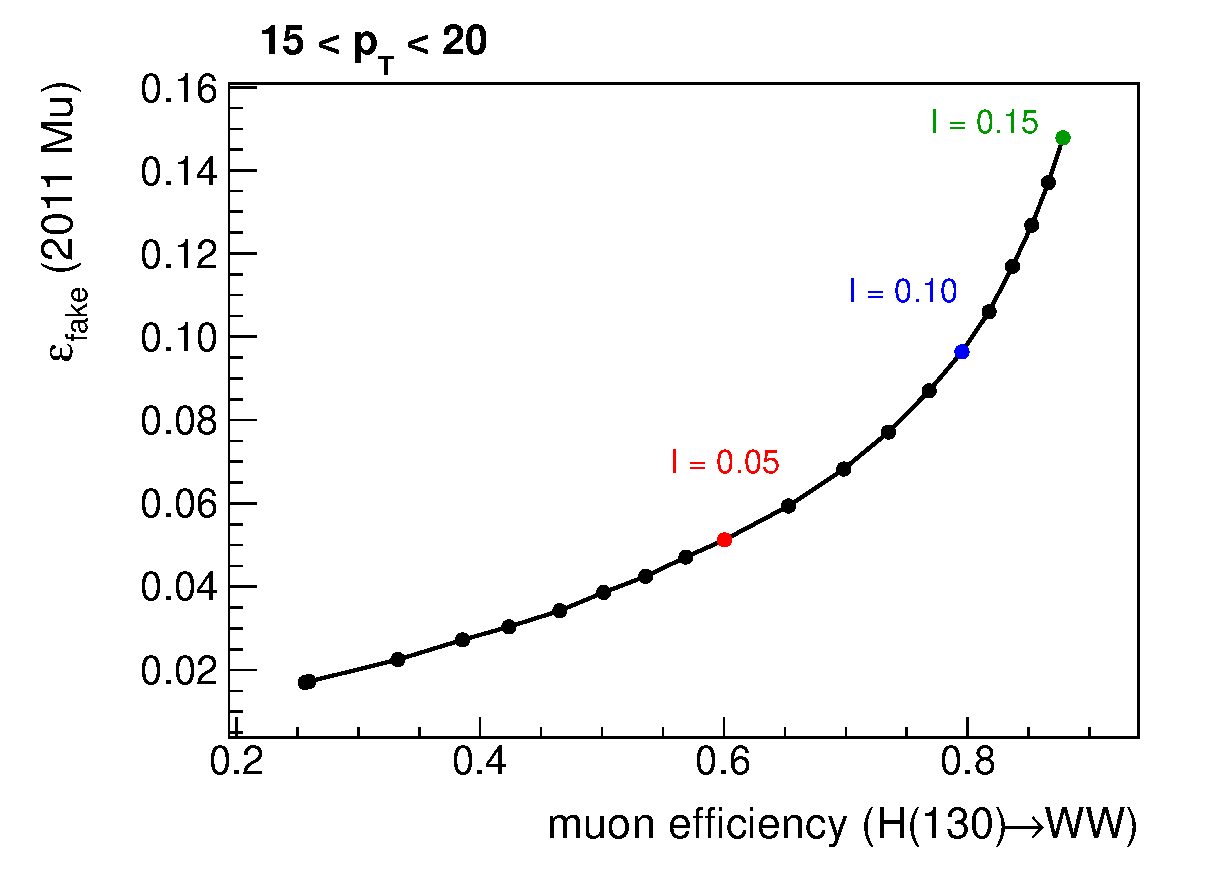
\includegraphics[scale=0.4]{figures/isoscan1.eps}
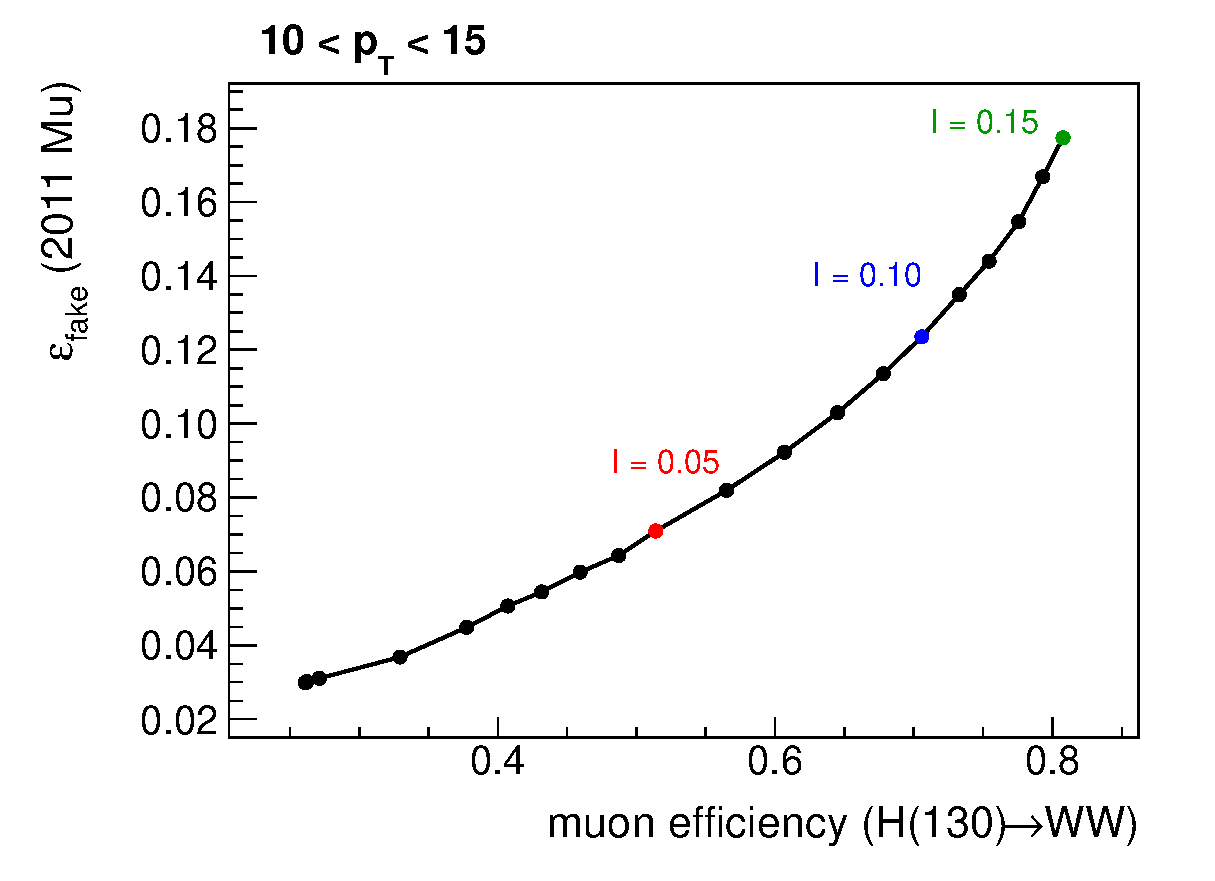
\includegraphics[scale=0.4]{figures/isoscan2.eps}
\caption{Fake rates versus signal muon efficiency for varying isolation cut in different $p_T$ bins.}
\label{fig:isoscan}
\end{center}
\end{figure}

The corresponding FOMs are shown in Figure~\ref{fig:isofoms}. Taking the FOMs and signal muon efficiencies into consideration, we choose a working point of $I<0.10$ for muons in the $10\:\GeVoverc < p_T < 20\:\GeVoverc$ range.
\begin{figure}[!htbp]
\begin{center}
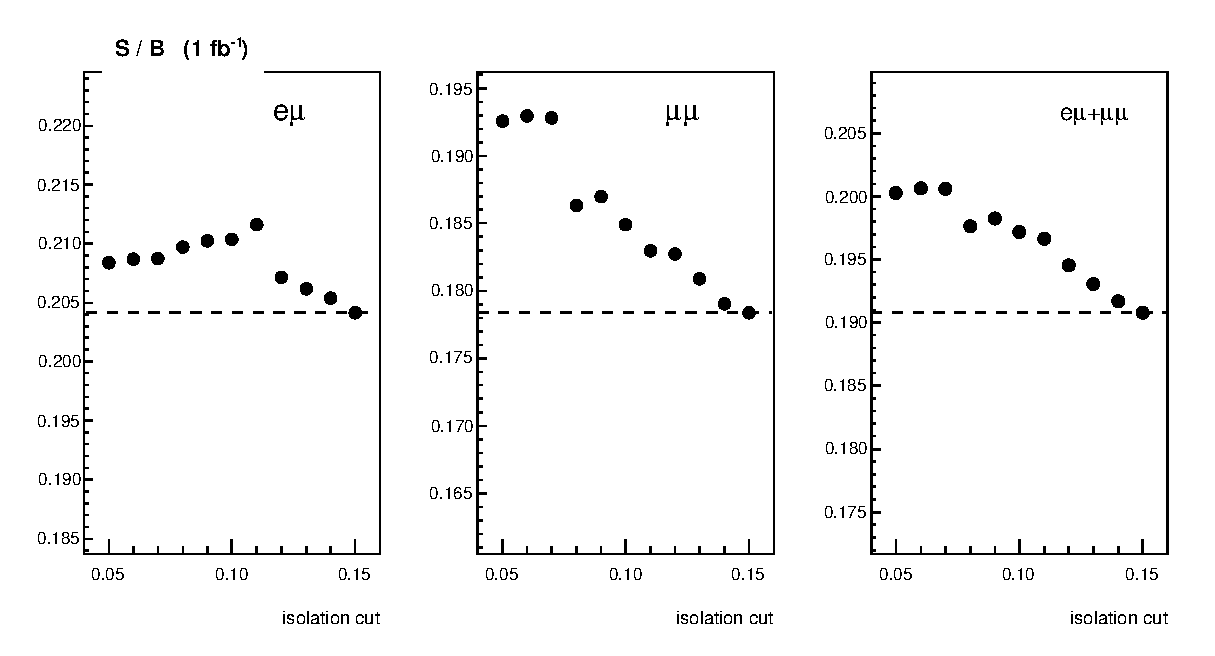
\includegraphics[scale=0.55]{figures/iso_fom1.eps}
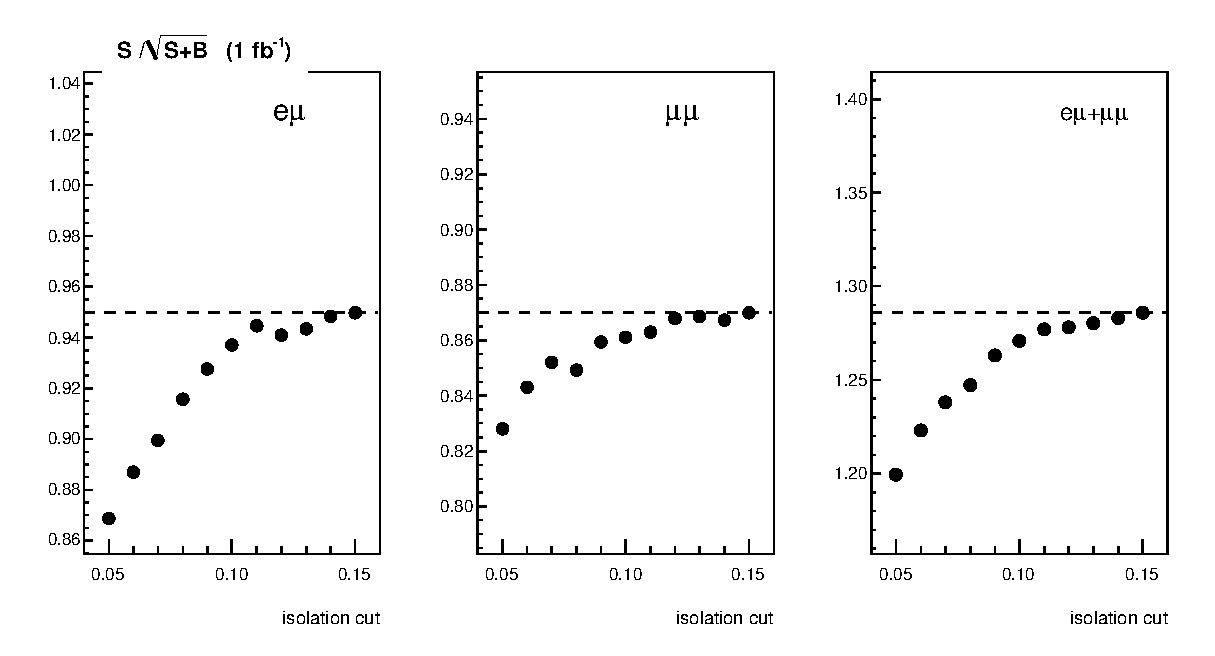
\includegraphics[scale=0.55]{figures/iso_fom2.eps}
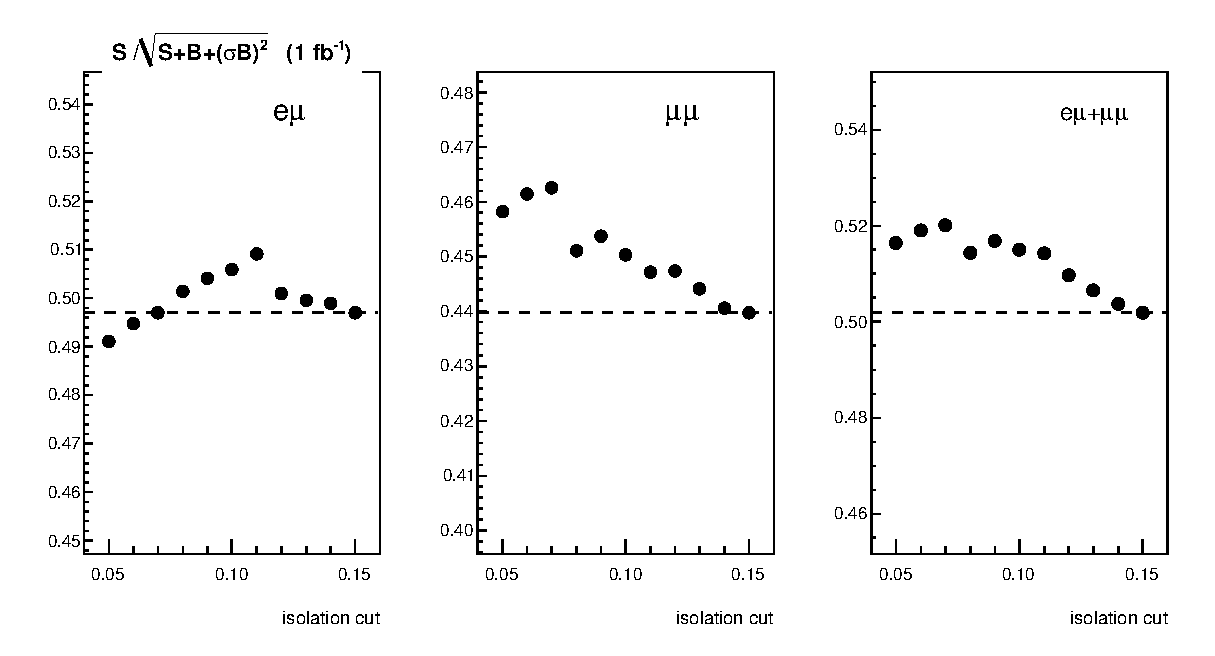
\includegraphics[scale=0.55]{figures/iso_fom3.eps}
\caption{Figures of merit for varying isolation cut.}
\label{fig:isofoms}
\end{center}
\end{figure}

\subsection{Impact Parameter}
We consider varying the impact parameter cut from the nominal value of $0.020\:$cm down to $0.005\:$cm. The curves of fake rate versus signal muon efficiency are shown in Figure~\ref{fig:ipscan}. It can be seen that $d_0$ and $d_0$-significance give very similar performance, so we decide to stay with using the $d_0$ variable as used in AN-10-344.

\begin{figure}[!htbp]
\begin{center}
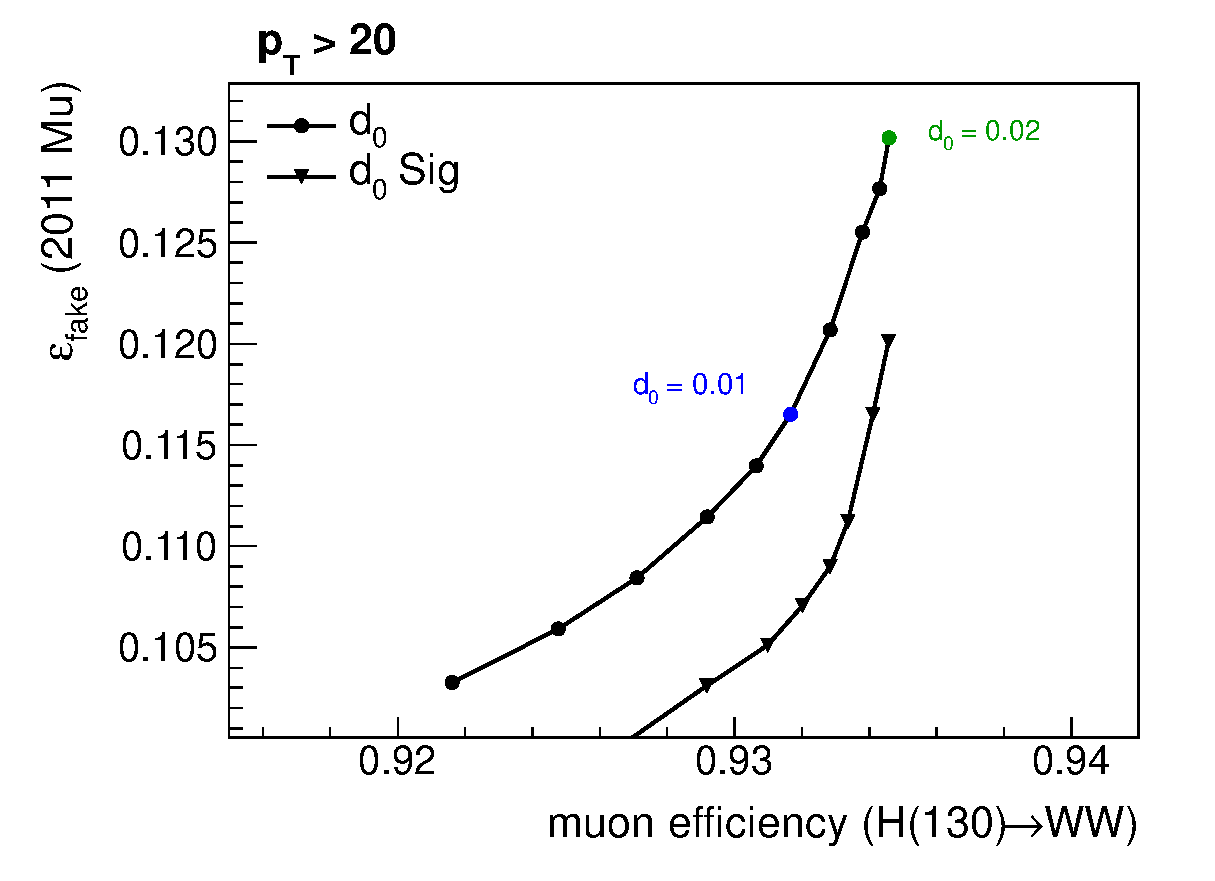
\includegraphics[scale=0.4]{figures/ipscan0.eps}
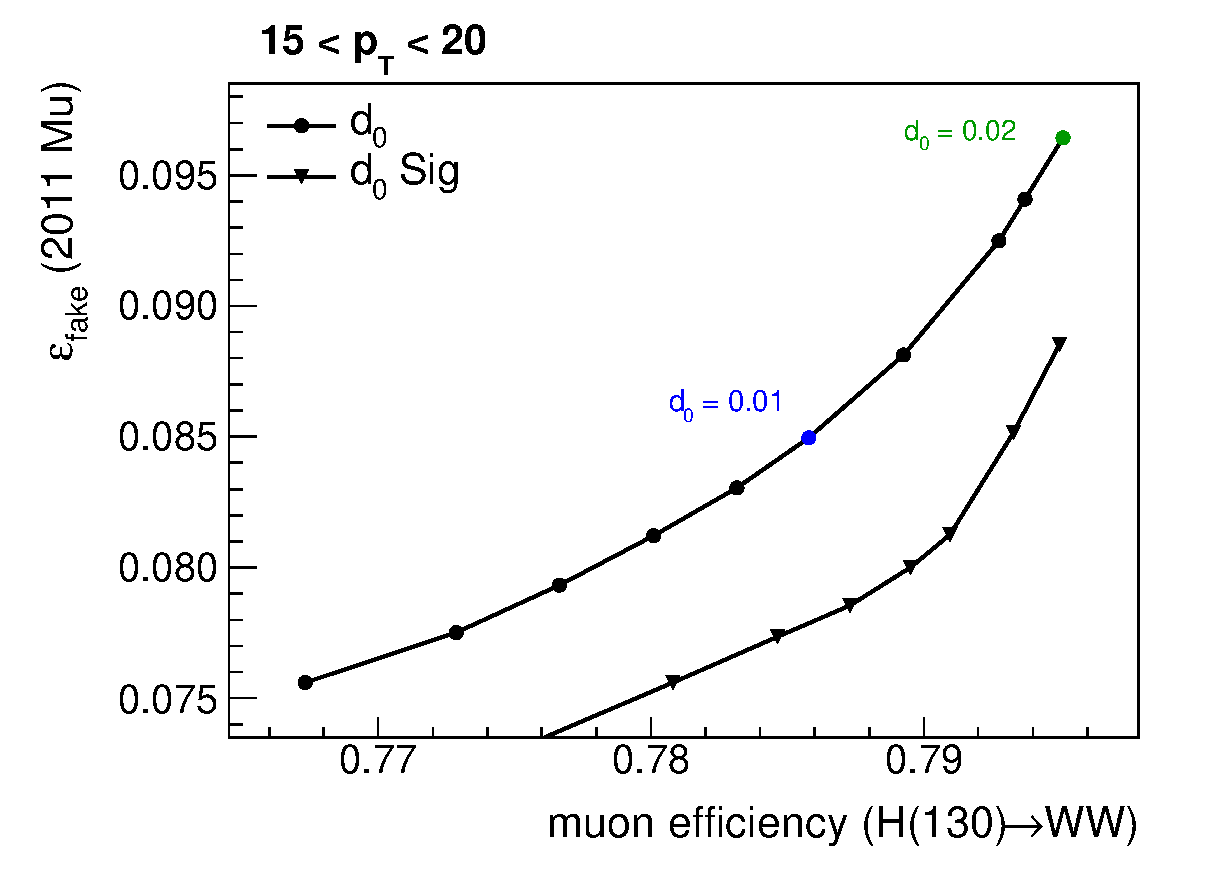
\includegraphics[scale=0.4]{figures/ipscan1.eps}
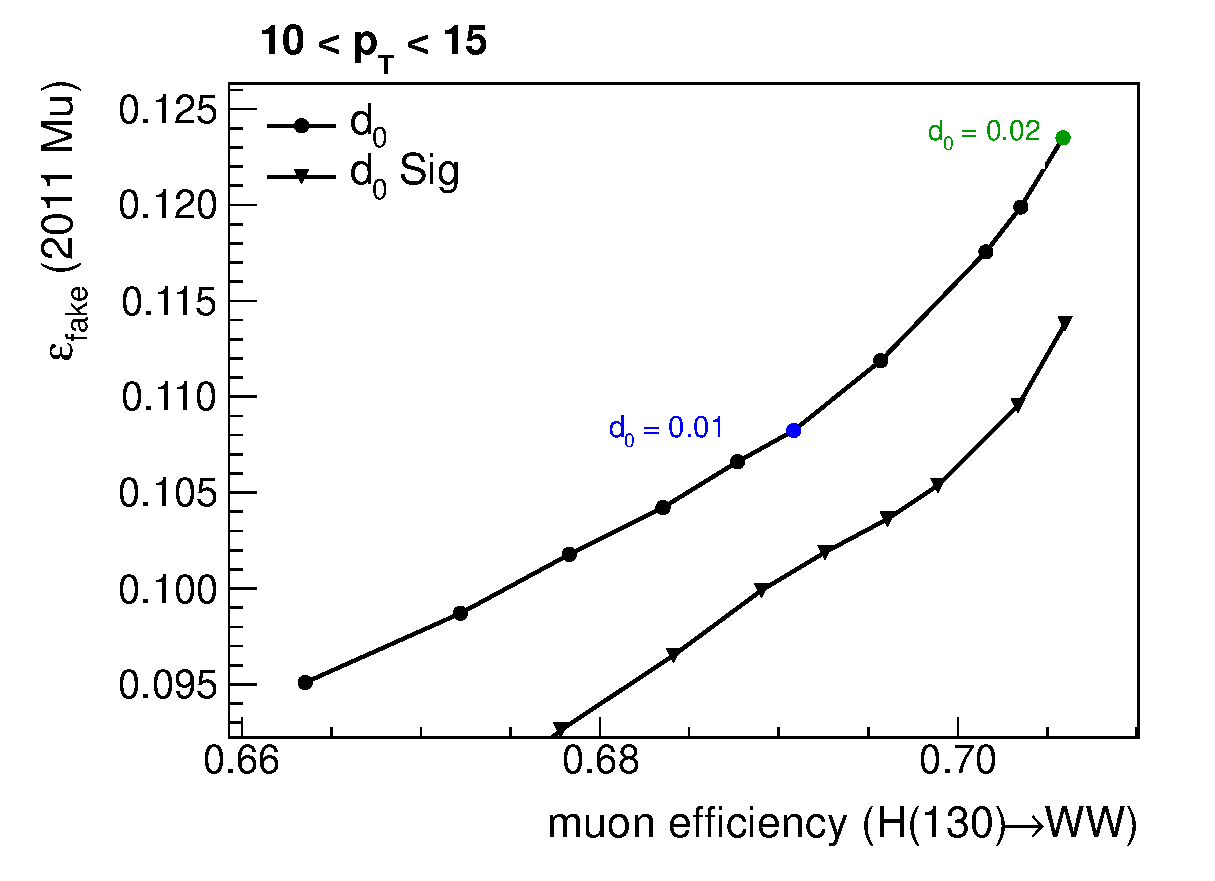
\includegraphics[scale=0.4]{figures/ipscan2.eps}
\caption{Fake rates versus signal muon efficiency for varying impact parameter cut in different $p_T$ bins.}
\label{fig:ipscan}
\end{center}
\end{figure}

The corresponding FOMs are shown in Figure~\ref{fig:ipfoms}. We choose a working point of $d_0<0.01\:$cm for muons in the $10\:\GeVoverc < p_T < 20\:\GeVoverc$ range.
\begin{figure}[!htbp]
\begin{center}
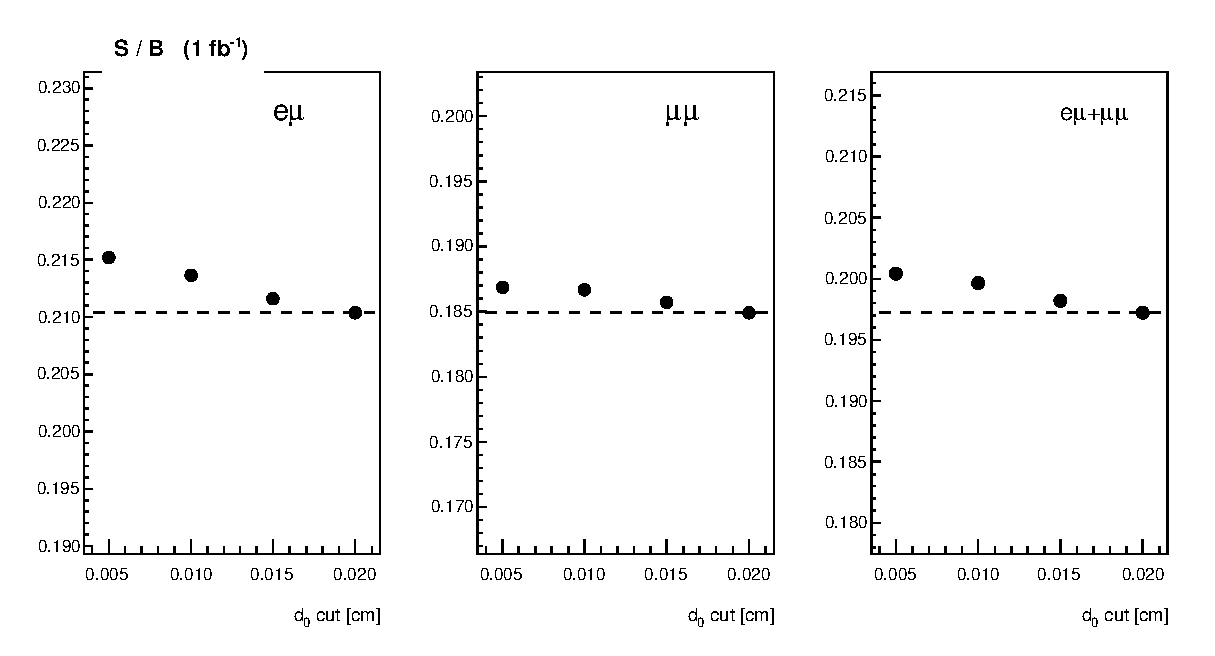
\includegraphics[scale=0.55]{figures/d0_fom1.eps}
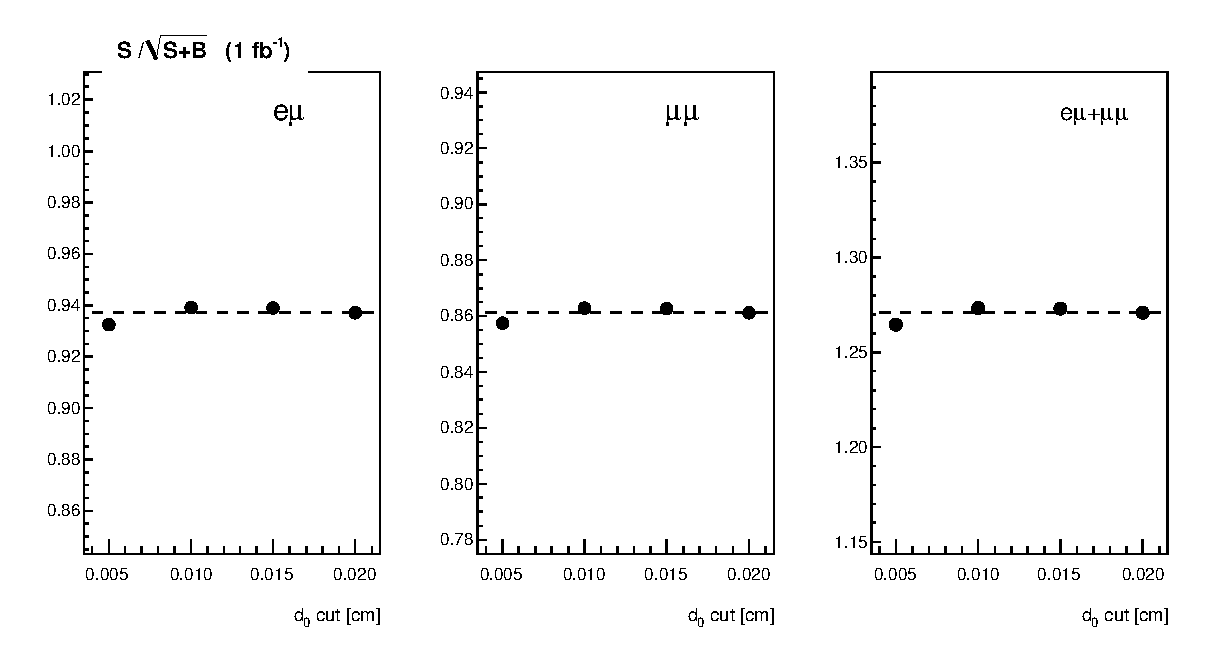
\includegraphics[scale=0.55]{figures/d0_fom2.eps}
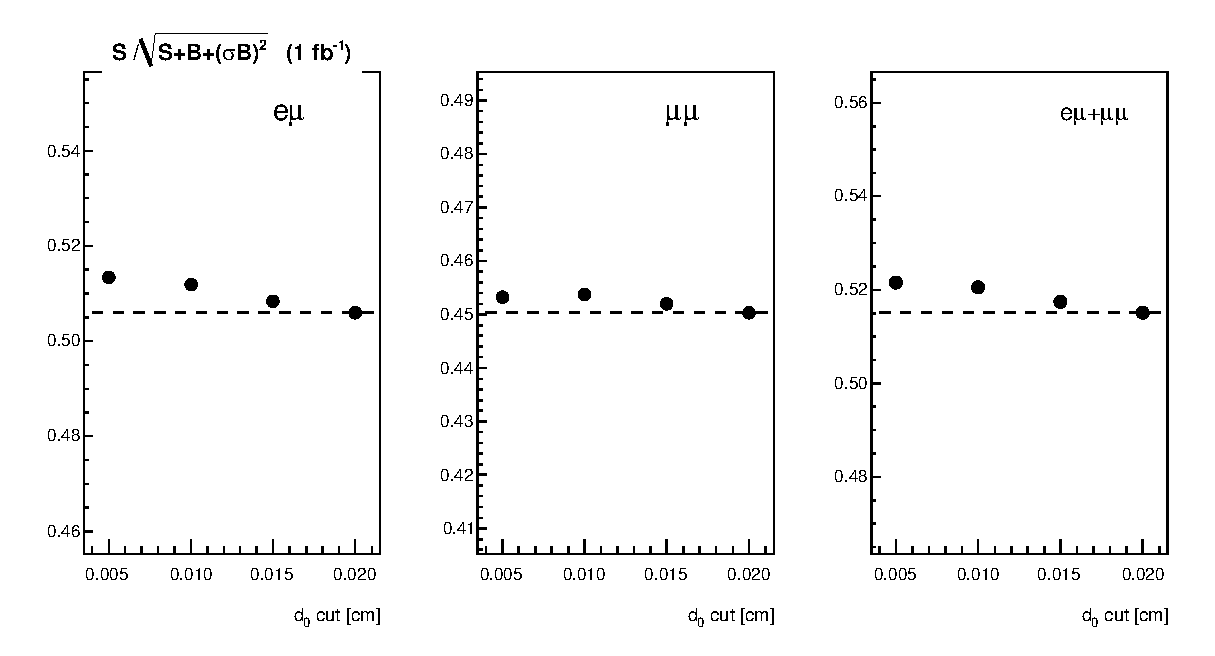
\includegraphics[scale=0.55]{figures/d0_fom3.eps}
\caption{Figures of merit for varying $d_0$ cut.}
\label{fig:ipfoms}
\end{center}
\end{figure}

\subsection{Results}
A summary of FOMs is provided in Table~\ref{tab:muidfom1}. Our chosen working point gives roughly a $5\%$ improvement in $S/B$ and a $4\%$ improvement in $S/\sqrt{S+B+(\sigma B)^2}$, while $S/\sqrt{S+B}$ suggests the performance degrades by about $1\%$.

\begin{table}[!htbp]
\begin{center}
\begin{tabular}{|l|c|c|c|}
\hline
	``20-20'' cuts & $e\mu$ & $\mu\mu$ & Both \\
\hline
$S/B$                       & $0.20$ & $0.19$ & $0.19$ \\
$S/\sqrt{S+B}$              & $0.64$ & $0.63$ & $0.90$ \\
$S/\sqrt{S+B+(\sigma B)^2}$ & $0.42$ & $0.41$ & $0.47$ \\
\hline\hline
	``20-10'' cuts & $e\mu$ & $\mu\mu$ & Both \\
\hline
$S/B$                       & $0.20$ & $0.18$ & $0.19$ \\
$S/\sqrt{S+B}$              & $0.95$ & $0.87$ & $1.29$ \\
$S/\sqrt{S+B+(\sigma B)^2}$ & $0.50$ & $0.44$ & $0.50$ \\
\hline\hline
	tight cuts & $e\mu$ & $\mu\mu$ & Both \\
\hline
$S/B$                       & $0.21$ & $0.19$ & $0.20$ \\
$S/\sqrt{S+B}$              & $0.94$ & $0.86$ & $1.27$ \\
$S/\sqrt{S+B+(\sigma B)^2}$ & $0.51$ & $0.45$ & $0.52$ \\
\hline
\end{tabular}
\caption{Summary of FOMs for the nominal cuts from AN-10-344 and our chosen working point.}
\label{tab:muidfom1}
\end{center}
\end{table}

The fake rate in the 2011 data before and after our chosen working point is shown in Figure~\ref{fig:mufakerate0}. The fake rate in bins of reconstructed vertices are shown in Figure~\ref{fig:mufakerate1}. The counted vertices are simply required to be valid and not fake. There is no apparent dependence of the fake rate on pile-up.

\begin{figure}[!htbp]
\begin{center}
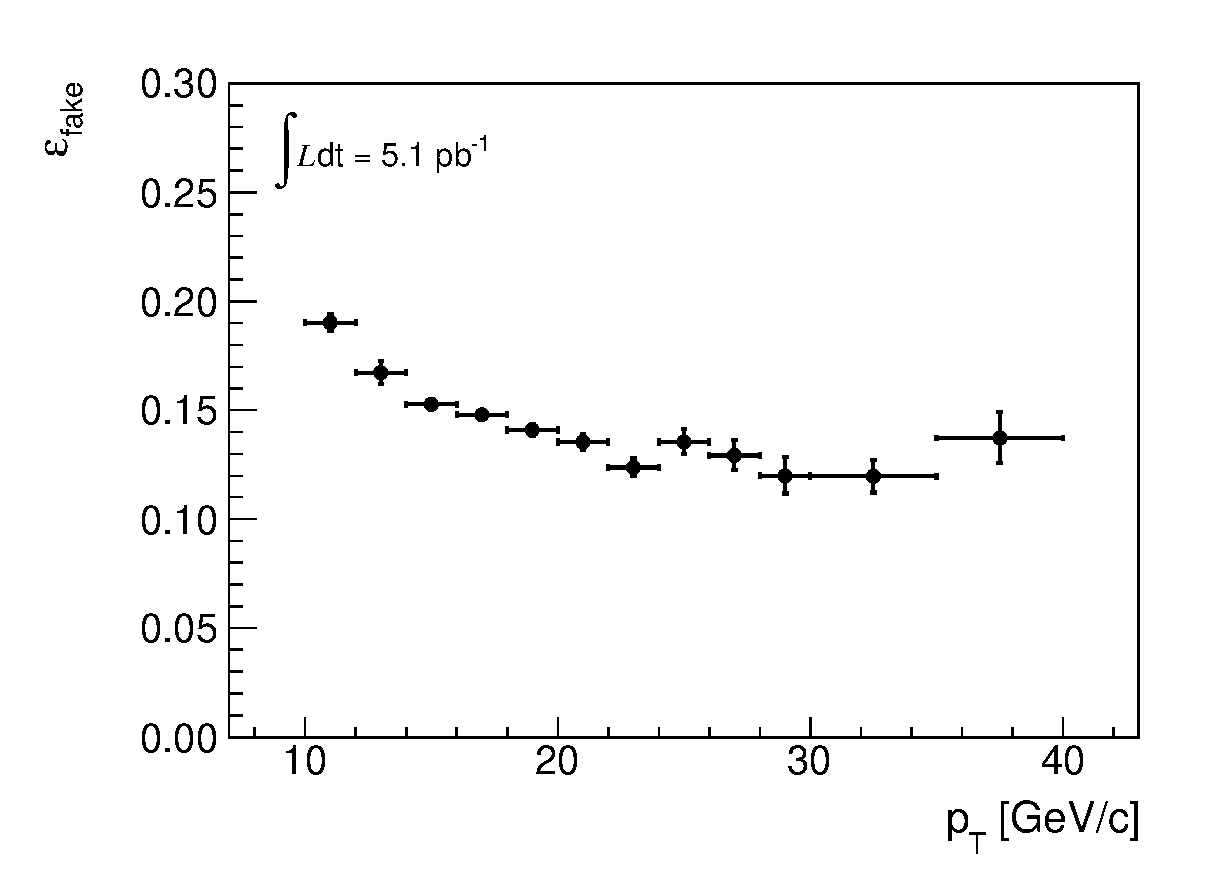
\includegraphics[scale=0.33]{figures/frpt_old.eps}
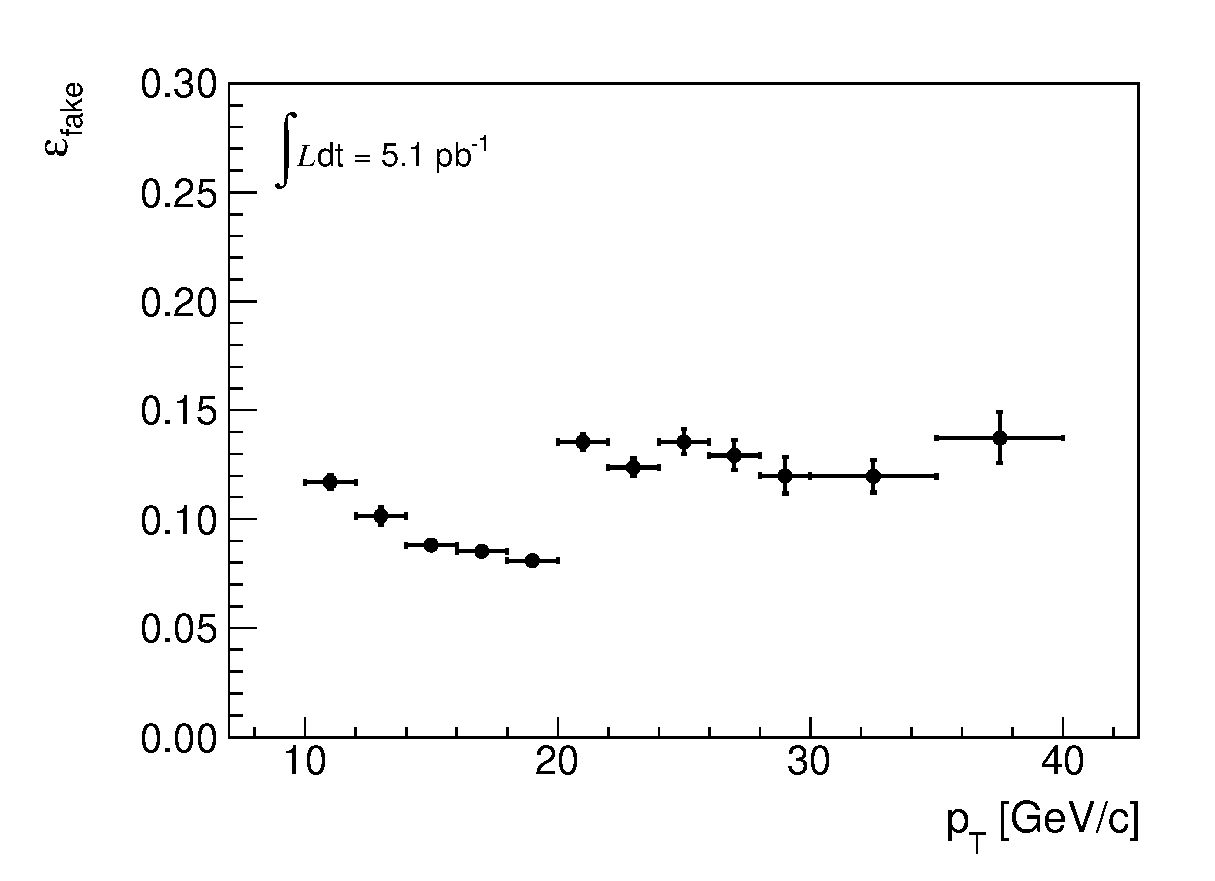
\includegraphics[scale=0.33]{figures/frpt_new.eps} \\
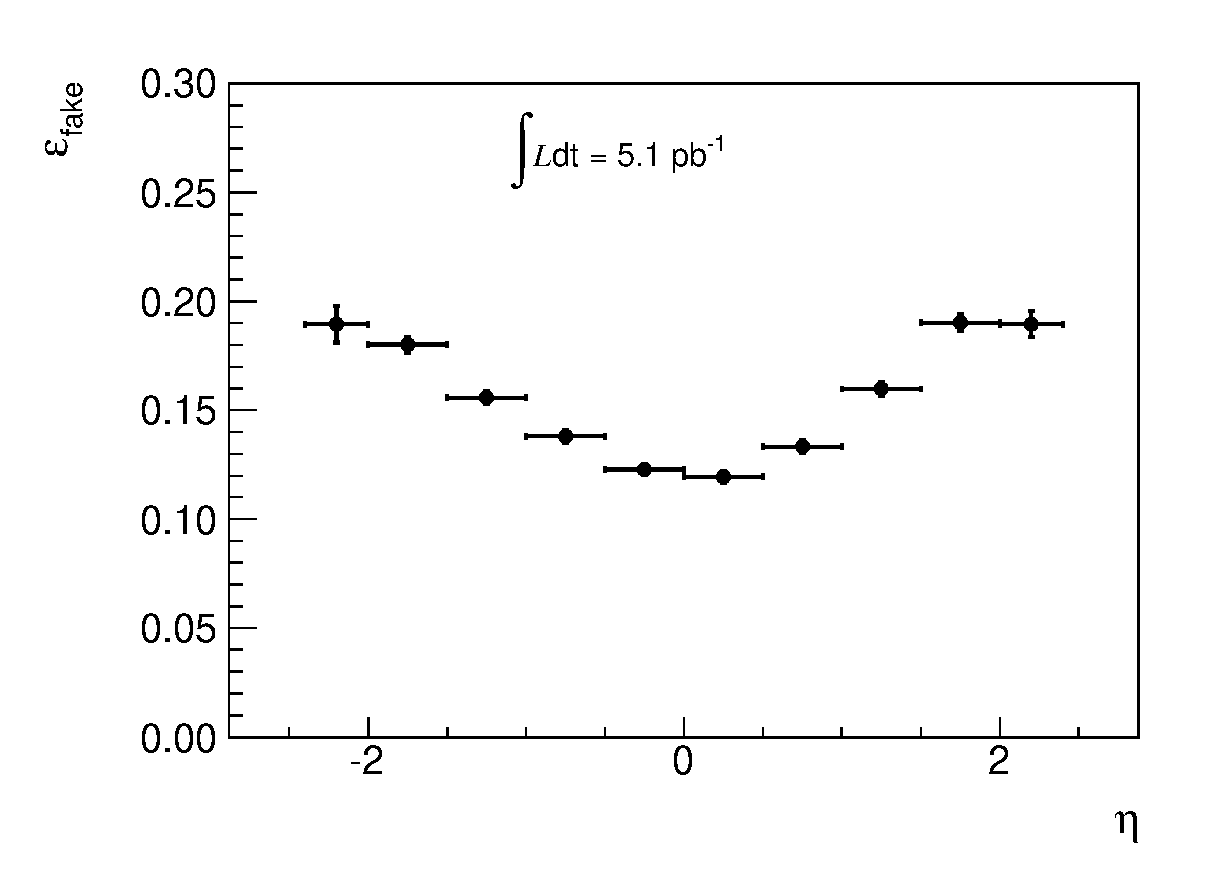
\includegraphics[scale=0.33]{figures/freta_old.eps}
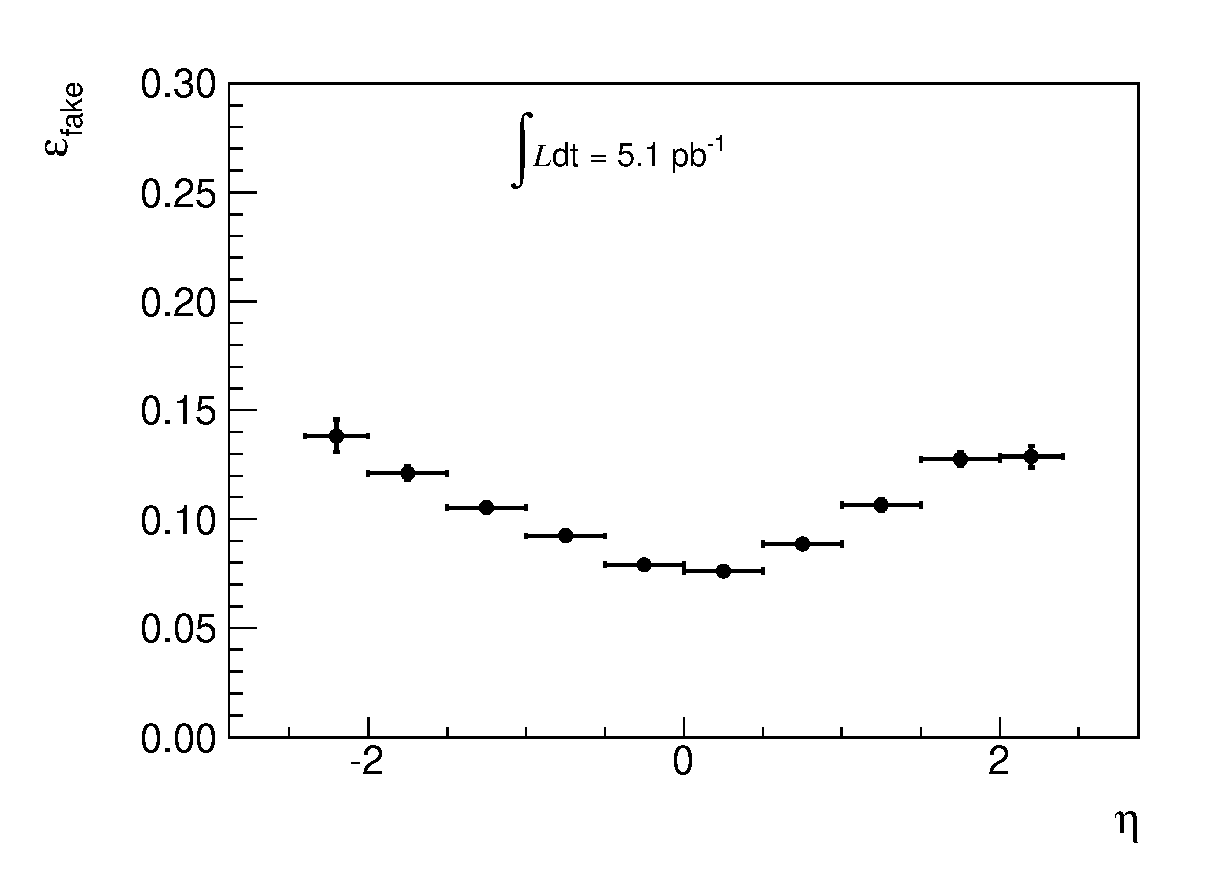
\includegraphics[scale=0.33]{figures/freta_new.eps}
\caption{Fake rate projections on $p_T$ (top) and $\eta$ (bottom) for the old muon identification selection (left) and the new selection with tighter isolation and $d_0$ (right).}
\label{fig:mufakerate0}
\end{center}
\end{figure}

\begin{figure}[!htbp]
\begin{center}
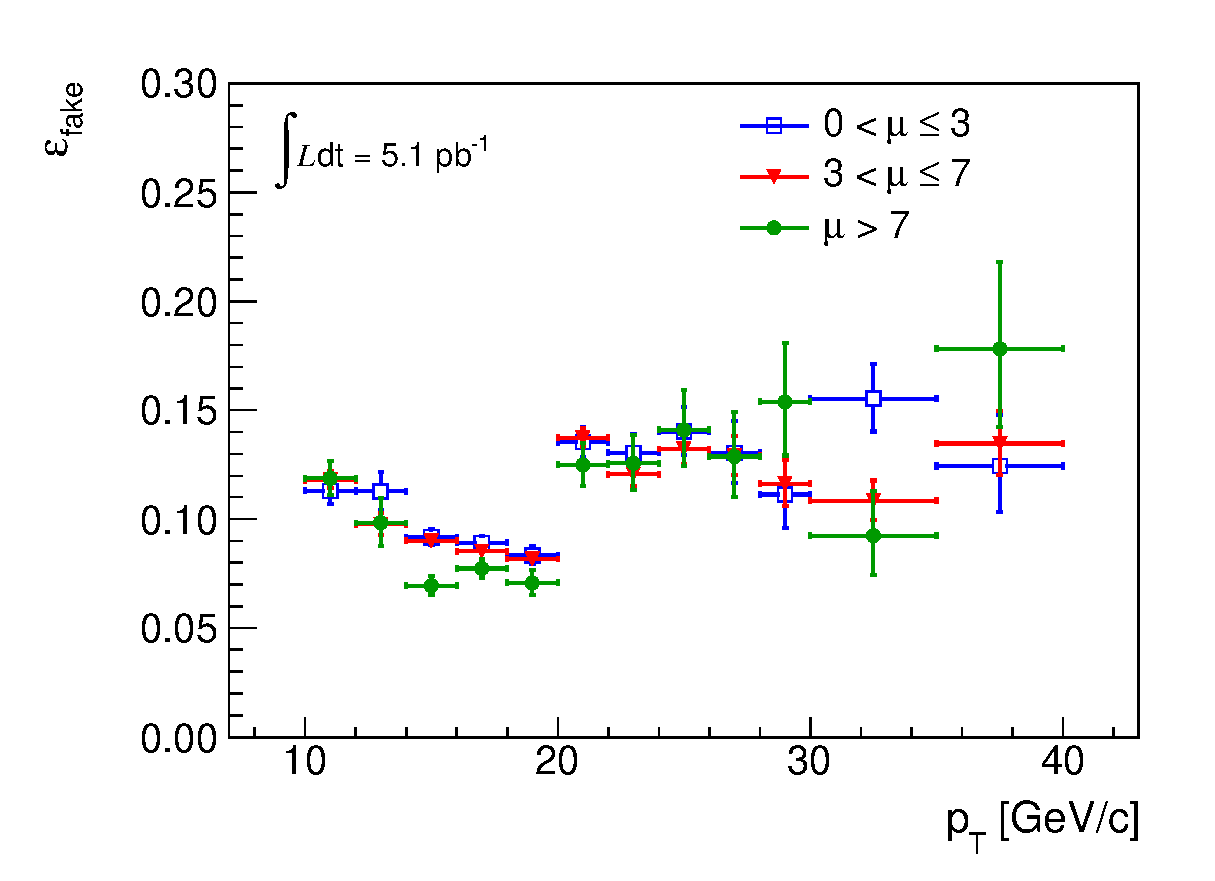
\includegraphics[scale=0.5]{figures/frpt_pu.eps}
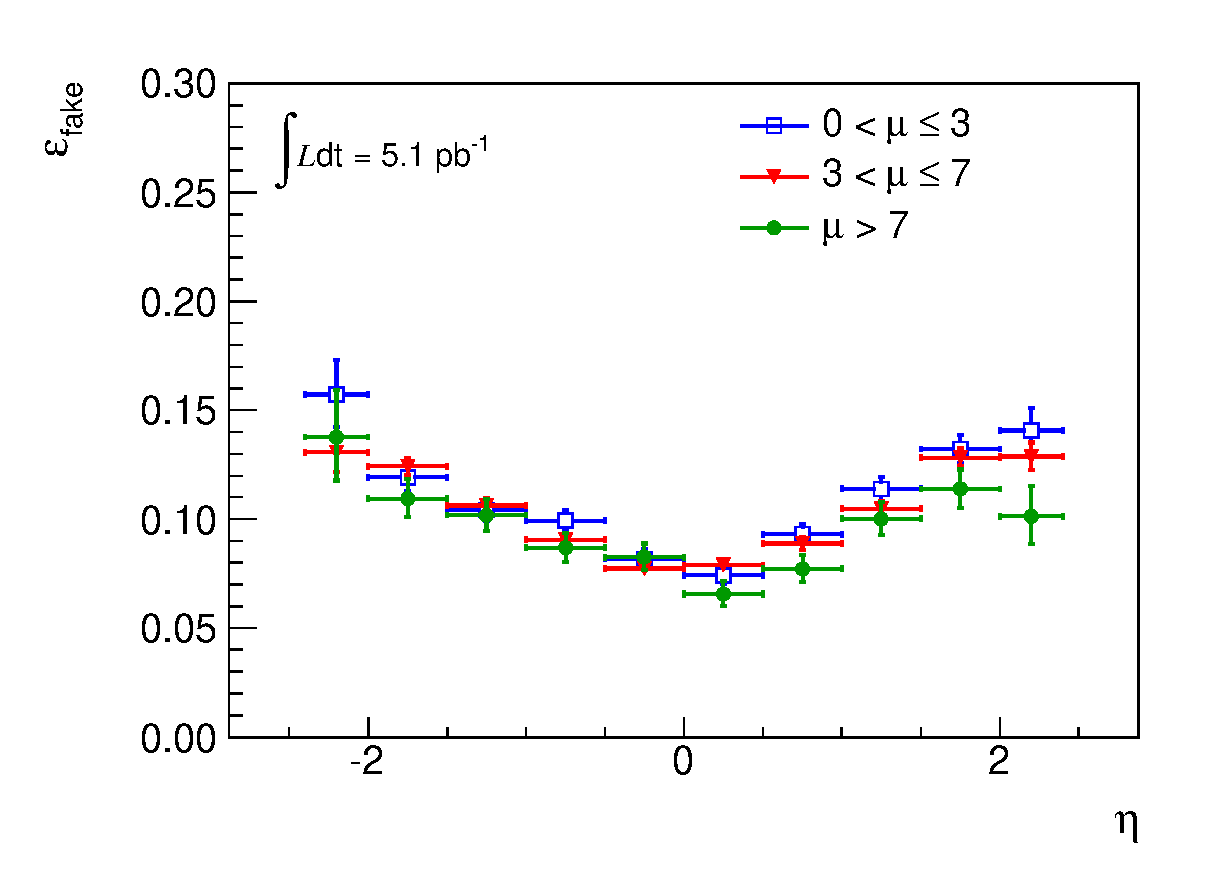
\includegraphics[scale=0.5]{figures/freta_pu.eps}
\caption{Fake rate projections on $p_T$ and $\eta$ in different bins of reconstructed vertices with the tighter selection.}
\label{fig:mufakerate1}
\end{center}
\end{figure}